\section{Sample Size Calculation}

\begin{frame}{}
  \begin{center}
    {\bf Part I -- Introductio and Motivation}
  \end{center}
\end{frame}

\subsection{Introduction}

\begin{frame}{Lecture Outline}

  In this course we talked several times about the necessity
  of collecting {\bf a sample}: A set of (multiple) observations
  that are used to calculate the value of interest.
  \bigskip

  However, up until now we have avoided talking about {\bf how big} this sample should be. This is the topic of today's lecture.\bigskip

  \begin{itemize}
    \item What is sample size?
    \item Why do we need to worry about it?
    \item What factors influence the choice of sample size?
    \item How to calculate the desired sample size?
  \end{itemize}

\end{frame}


\subsection{Motivation}

\begin{frame}{Why take samples?}{Review: Noise Factors}
  As we discussed before, the result of an experiment is affected by several factors, some of which are unknown, or difficult to control.\bigskip

  Because of these {\bf Noise Factors}, sometimes there will be a small variance in the result of repeated experiments. To measure this variance, and take it into account for our analysis, we repeat the experiment several times, and gather those repetitions into a {\bf sample}.\bigskip


  \begin{columns}
    \column{0.2\textwidth}
      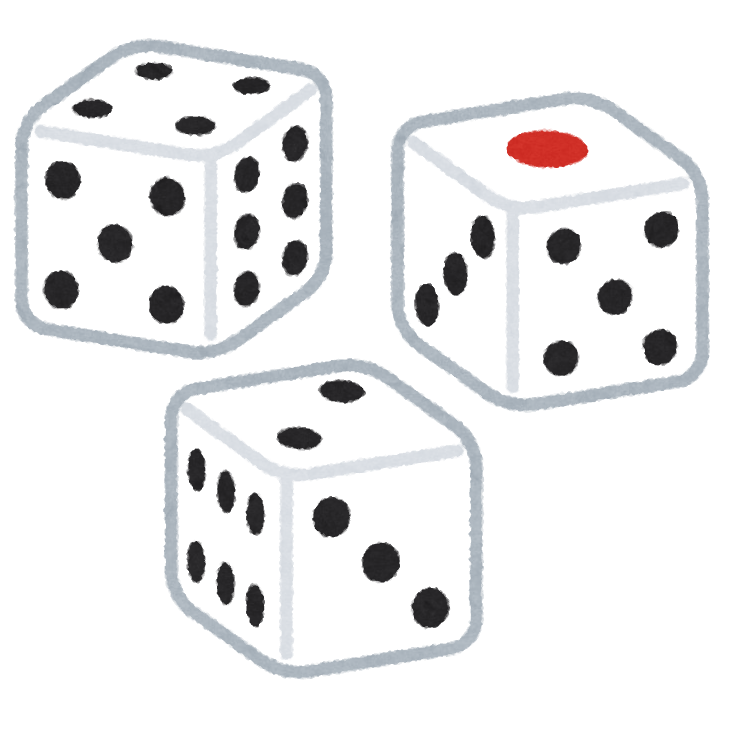
\includegraphics[width=\textwidth]{../img/irasutoya_dice}
    \column{0.8\textwidth}
      {\bf For example:} The true mean of throwing three dice and adding their values is {\bf 10.5}. However, every time we throw the dice, the result will be a bit different.
  \end{columns}
\end{frame}

\begin{frame}{Why take samples}{What are repetitions good for?}

  - Estimator Variance is based on the sample error
  - Test Confidence
  - Test Power

\end{frame}


% - Power and Sample size, what it is, and why it matters?
%   - Power: probability of type II error
%   - Sample size: number of observations, related to experiment robustness
%     - When sample size goes up: In general, error of estimators (mean, deviation) goes down
%     - The deviation of the data itself does not go down!
%       - Dice example: estimation of the mean goes down, but the error of one dice remains.
%       - So this allows us to separate "sampling error" from "natural deviation of the observed phenomenon"
%     - cost of experiment goes up!

%%%% Is sample size always good?
\begin{frame}{Is "the more the merrier" the answer?}

  From the previous slide, we could think that "the more observations the better", but that is not quite right.\bigskip

  \begin{itemize}
    \item As we saw in the first class on hypothesis testing, it is possible to
    reduce $p$ to arbitrary values by largely increasing $n$.\bigskip

    \item On the other hand, increasing the number of observations can be costly (financial costs, time costs, human costs, etc)\bigskip

    \item The choice of $n$ influences how the data will be selected and analyzed, so it is helpful to know this value during experiment design;
  \end{itemize}\bigskip

  Because of this, we are interested in a more formal way to define the number of observations necessary in an experiment;
\end{frame}




\subsection{Fixed Sample Size}

% - How to determine sample Size
%   - When sample size is chosen for you:
%     - Experiment cost
%     - Experiment restriction
%   - What can we do, when we cannot choose sample size?
%     - Cancel the experiment? Not necessarily
%     - We can measure the power of the experiment, and determine how much we can rely on the results
%     - We can improve the power of an experiment by changing delta.

\begin{frame}{Experiment Power}{Budget Constrained case}
  When an experiment is constrained by budget (not enough time,
  not enough money, etc), we might not have a choice of sample size.\bigskip

  However, even in this cases the calculation of sample size is important,
  because it can be used to give us information about {\bf experiment power}.\bigskip

  The power of an experiment is an expression of the probability of {\bf Type II errors} (False Negatives). It tells us {\bf how sensitive our experiment is to actually find the effect that we are looking for}.\bigskip

  If our experiment is budget-constrained, a power analysis may tell us if the experiment is not useful at all, or if we need to settle for a larger minimum effect.
\end{frame}

\begin{frame}{Sample size and Type-II error}
  The probability of Type-II error can be easily (and often wrongly) evaluated \textit{a posteriori}, but its definition \textit{a priori} requires some care; \bigskip

  Given a desired test, its power is essentially a function of 4 elements:
  \begin{itemize}
    \item Actual size of the difference;
  	\item Variability of the observations;
  	\item Significance level;
  	\item Sample size.
  \end{itemize}\bigskip

  The experimenter generally has very little control over the first two.\\
  But they can be estimated.
\end{frame}

\begin{frame}{Sample size and Type-II error}
  {Estimating Experimental Power}
  A strategy for estimating an effective lower bound for the power of a test includes a definition of an \textit{minimally interesting effect} $\delta^*$.
  \bigskip

  This value must be derived from technical and scientific knowledge about the phenomenon or system under experimentation.
  \bigskip

  \begin{block}{}
  \centering It is essential to have a good understanding of the field in which the experiment will be conducted.
  \end{block}\bigskip

  Once $\delta^*$ is defined, the experimenter can obtain an estimate of the variability of observations (e.g., by a pilot study), which can then be used to obtain an approximate power value for the experiment;
\end{frame}

%=====

\begin{frame}{Sample size and Type-II error}{Some considerations}
  Having obtained this estimation of the Type-II error probability, one can run his/her experiment with a better understanding of its ability to detect effects of interest.\bigskip

  The test will have lower power for differences smaller than $\delta^*$, but these differences are below the minimally interesting effect; any effect greater than $\delta^*$ will result in a higher power for the test;\bigskip

  This technique is most useful to compute the required sample size for the   experiment.
\end{frame}

\begin{frame}[fragile]{Sample size and Type-II error}{Example of power calculation}
Consider an one-sample experiment with the following parameters: Alternate hypothesis is one-sided, sample size is 10, $\delta^*=0.5$, estimate of standard deviation is $\sigma=1$, desired significance $\alpha=0.01$.\medskip

What is the power of this experiment?

{\smaller
\begin{verbatim}
> power.t.test(n = 10, delta = 0.5, sd = 1, sig.level = 0.01,
+        type = "one.sample", alternative = "one.sided")

One-sample t test power calculation
n = 10
delta = 0.5
sd = 1
sig.level = 0.01
power = 0.1654013           <- Power = 0.16 - Very low!
alternative = one.sided        High chance for false negatives
                               *For this effect size*
\end{verbatim}}
\end{frame}


\subsection{}
\begin{frame}{}
  \begin{center}
    {\bf Part II -- Sample Size Calculation}
  \end{center}
\end{frame}


\subsection{The magic number "30"}

% - Sample size = 30
%   - Why do we see this value so often?
%     - Because in general, it guarantees that the estimator will be normally distributed.
%   - Is this a bad or good value?
%     - (There are no bad or good values, there are things the value gives you, or not give you)
%     - As sample size 30 will in general guarantee that your mean estimator will follow a normal distribution, except in extreme cases
%     - But this is all that it guarantees you! It does not guarantee anything
%       about the alpha or beta of the experiment.
%     - If your variation is too high, you will need more samples
%     - but if your variation is low (or you have good pairs), then
%       you are wasting money / time / other costs with too many experiments.
%     - You need to do power calculations, even if you use N = 30
%     - Also, you need to guarantee other assumptions

\begin{frame}{"We repeated each experiment 30 times"}
  In Computer Science papers, it is common to see papers stating that they repeated computational experiments "30 times" (or sometimes 20). Where does this rule of thumb comes from?\bigskip

  The Central Limit Theorem (CLT) states that the distribution of sample means tends to follow a normal distribution. This effect can be observed even on means of much smaller samples for well-behaved distributions. However, in general the CLT will hold for $n > 30$, except for extreme cases of non-normality;\bigskip

  As many testing procedures require the assumption of normality from the underlying distribution, an "oral tradition" of using $n=30$ began in some CS groups. But it is much better to try to actively identify the correct sampling size for your experiment.
\end{frame}

\begin{frame}{When is sample size 30 not appropriate?}
  \begin{itemize}
    \item The underlying distribution of the population is very well behaved;
    \item Your planned analysis does not require assumption of normality; \bigskip

    \item You are comparing samples with very different variants; \bigskip

    \item Your budget does not allow for sample size equal to 30;
    \item Your experiment is dangerous (example, drug tests), and you want to minimize the number of experiments;
  \end{itemize}\bigskip

  All of these cases are strong reasons for a more explicit sample size calculation;
\end{frame}


\subsection{Sample Size Calculation}

% - Sample size calculation
%   - sample size calculation for single sample test
%   - sample size calculation for post-hoc multi-sample test
%   - Methods for z tests, methods for post-hoc tests
% - Be careful with sample size calculations:
%   - Pseudo-replication (it is not the sample size the matters, but how you choose it.)
%     - An extreme example: We develop an algorithm to solve optimization problems.
%     - The optimization problems have "Types", "Sub-types", and "Sub-Sub types"
%     - We are interested

\begin{frame}[fragile]{Sample size and Type-II error}
{Example of sample size calculation}

With only $n=10$ samples, the experiment is {\bf underpowered}. What is the smallest sample size needed to obtain a desired power of $0.85$?

{\smaller
\begin{verbatim}
> power.t.test(power = 0.85, delta = 0.5, sd = 1,
               sig.level = 0.01,
               type = "one.sample", alternative = "one.sided")

One-sample t test power calculation
n = 47.98044                      <-- Round this value up!
delta = 0.5
sd = 1
sig.level = 0.01
power = 0.85
alternative = one.sided
\end{verbatim}}

We need at least 48 observations to detect a one-sided deviation of 0.5 or more on the mean  with a power level of $0.85$.
\end{frame}

\subsection{Sample Size for Two Means}

%% TODO: Add the experimental context here
\begin{frame}{Sample Size Calculation}{Example for Two Means}

Let's consider a more general example, where we are comparing two means with the following experimental characteristics:\bigskip

\begin{itemize}
  \item Desired significante $\alpha = 0.05$
  \item Desired power: $(1-\beta) = 0.8$;
  \item Minimally relevant effect size (MRES): $\delta^* = 15$
  \item Variances of the samples: $\sigma_1, \sigma_2 = ?$
\end{itemize}\bigskip

From these specifications, we can obtain the required sample sizes.
\end{frame}

\begin{frame}{Sample Size Calculation}{Two means with equal variances}

For the specific case of approximately equal variances, the optimal sample size ratio is $n_1 = n_2 = n$, with:

\begin{equation*}
n \approxeq 2\left(\frac{t^{(2n-2)}_{\alpha/2}+t^{(2n-2)}_{\beta}}{d^*}\right)^2
\end{equation*}

where $d^* = \delta^*/\sigma$ is the (standardized) minimally interesting effect size; and $t^{(2n-2)}_{\alpha/2}$ and $t^{(2n-2)}_{\beta}$ are the $\alpha/2$ and $\beta$ quantiles of the $t^{(2n-2 )}$ distribution.\bigskip

Can we do this calculation? Or is there something missing?

\end{frame}

\begin{frame}{Sample Size Calculation}{How to obtain the variance estimate}

These formulas are very convenient, but leave us with a riddle: we need variance estimate in order to calculate the sample size, but we need observations to be able to estimate the variance!\bigskip

There are a few ways to proceed in this case. The most practical are:

\begin{itemize}
  \item Use process knowledge or historical data to obtain an (initial) estimate of the variance;
  \item Use a standardized MRES to calculate sample size;
  \item Perform a pilot study and collect samples to estimate the variance.
\end{itemize}\bigskip

Each approach has its own advantages and drawbacks.
\end{frame}

\begin{frame}{Sample Size Calculation}{Pilot Study}
If no information is available to estimate the variance, a pilot study must be performed to obtain this value. The sample size required for this pilot study is given by:

\begin{equation*}
n_{\mbox{\textit{pilot}}}\approx 2\left(\frac{z_{\alpha_n/2}}{e_{n}}\right)^2
\end{equation*}

\noindent where $(1-\alpha_{n})$ is the desired confidence level for the sample size estimate of the main study, and $e_n$ is the maximum relative error allowed for the sample size.\bigskip

This calculation can yield some scarily large sample sizes for a pilot study (much larger than would be actually required for the main study itself), so use this with caution.
\end{frame}


\begin{frame}{Calculation of Sample Sizes}{Case of Known Standard Deviation}
Suppose that the engineer uses data available from the system manuals, as well as historical measurements, to estimate a reasonable upper bound for the common standard deviation as $\sigma \approxeq 15$.\bigskip

Assuming that equal sample sizes are desired, we can simply use the formula:

\begin{equation*}
n \approxeq 2\left[\left(t^{(2n-2)}_{\alpha/2}+t^{(2n-2)}_{\beta}\right)\frac{\sigma}{\delta^*}\right]^2
\end{equation*}
\vfill

\hfill Easy, right?
\end{frame}

\begin{frame}{Calculation of Sample Sizes}{Case of Known Standard Deviation}

The last problem we have to solve is that the values of $t^{(2n-2)}_{\alpha/2}$ and $t^{(2n-2)}_{\beta}$ are also dependent of $n$, which makes the sample size equation transcendental in $n$.\bigskip

We can solve that by using an initial estimate of $t^{(2n-2)}_{\kappa}\approx z_{\kappa}$, and iterating until we find the smallest $n$ that satisfies:

\begin{equation*}
  n \geq 2 \left(\frac{\hat{\sigma}}{\delta^*}\right)^2\left(t_{\alpha/2}+t_{\beta}\right)^2
\end{equation*}
\end{frame}


\begin{frame}[fragile]{Calculation of Sample Sizes}
{Case of Known Standard Deviation}

In practice, there are many sample size calculators in statistical software. But it is important to known the idea behind the calculation, for when we find ourselves in special situations.

{\smaller
\begin{verbatim}
> ss.calc <- power.t.test(delta       = 15,
                          sd          = 15,
                          sig.level   = 0.05,
                          power       = 0.8,
                          type        = "two.sample",
                          alternative = "one.sided")

Two-sample t test power calculation
n = 13.09777       <- NOTE: n is the number in *each* group
delta = 15
sd = 15
sig.level = 0.05
power = 0.8
alternative = one.sided
\end{verbatim}}
\end{frame}

% \begin{frame}{Case of Two Means -- Unequal Variance}
%
% The two-sample Welch t-test for considering unequal variances is usually the first test of choice, since it drops one (often inconvenient) assumption, at a very small cost in terms of power.\bigskip
%
% Calculating sample sizes for the general case (unequal variances, unequal sample sizes) is not particularly difficult, and can be done for either a \textit{balanced} case (i.e., $n_1 = n_2 = n$) or an optimal, \textit{unbalanced} case (in which $n_1 \neq n_2$).\bigskip
%
% For the unbalanced case, it is not particularly difficult to prove that the optimal allocation of observation is to keep:
% $$\frac{n_1}{n_2} = \frac{\sigma_1}{\sigma_2}$$.
%
% (if a good estimate of the ratio of variances is available, of course).
% \end{frame}

\begin{frame}{Comparison of two means -- Paired design}
Paired designs can require smaller sample sizes for equivalent power in cases where the {\bf between-units variation} is relatively high, and the {\bf in-unit variation} is relatively homogeneous.\bigskip

More specifically, if the within-level variation is given by $\sigma_\epsilon$ and the between-units variation is $\sigma_u$, we have that, for large enough $N$\\(e.g., $N\geq 10$),

\begin{equation*}
\frac{N_{\mbox{\tiny unpaired}}}{N_{\mbox{\tiny paired}}}\approx\sqrt{2\left[\left(\frac{\sigma_u}{\sigma_\epsilon}\right)^2+1\right]}
\end{equation*}
\end{frame}


% % Equivalence testing
% \begin{frame}{Sample size for Equivalence of a single mean}
% Sample sizes for testing equivalence of a single mean can be derived using essentially the same considerations used for the usual tests. In the case of a single sample:
%
% \begin{equation*}
% n\geq\left(\frac{\left(t_{\alpha}+t_{\beta}\right)\hat{\sigma}}{\delta^* - \Delta\mu}\right)^2
% \end{equation*}
% \bigskip
%
% As in the previous cases, iteration is needed to solve for $n$ (since the quantiles of the t distribution depend on $n$). Use $t_x$ = $z_x$ for the first iteration.
% \end{frame}
%
% \begin{frame}
% {Sample size for Equivalence of two means}
%
% Sample size for the $n_1 = n_2 = n$ case can be approximated based on the Zhang formula.
% $$n \geq \left(t_{\alpha;\nu}+t_{(1-c)\beta;\nu}\right)^2\left(\frac{\hat{\sigma}_1^2+\hat{\sigma}_2^2}{\delta^*-\Delta\mu^*}\right)^2$$
%
% \noindent with $\Delta\mu^*<\delta^*$ as the maximum real difference between the two means for which a power of $(1-\beta)$ is desired, and:
% $$c = \frac{1}{2}\exp\left(-7.06\frac{\Delta\mu^*}{\delta^*}\right)$$
% \end{frame}

\subsection{Sample Size for Multiple Means}

\begin{frame}{Sample size formulas for ANOVA}
If one is interested in calculating the required sample size for the ANOVA procedure (without worrying about the eventual post-hoc testing), the formulas are almost as simple as those used for the t tests.\bigskip

Essentially, the power/sample size calculations for the ANOVA boil down to the equality:

\begin{equation*}
F_{(1-\alpha)} = F_{\beta;\phi}
\end{equation*}

with both $F$ distributions having $(a-1)$ degrees of freedom in the numerator and $a(n-1)$ in the denominator. The noncentrality parameter $\phi$ is given by:

\begin{equation*}
\phi = \frac{n\sum\limits_{i=1}^{a}\tau_i^2}{\hat{\sigma}^2}
\end{equation*}
\end{frame}

\begin{frame}{Sample size formulas for ANOVA}

To ilustrate the sample size calculation procedure, imagine an experimental design with $a = 4,\ \alpha = 0.05,\ \hat{\sigma} = 7$, and suppose that the researcher wants to be able to detect whether any two means present differences of magnitude $\delta^* = 12$ with power $(1-\beta)=0.8$.\bigskip

Under these conditions, two scenarios tend to be of interest: the first is if we have two levels biased symmetrically about the grand mean, and all the others equal to zero:

$$ \tau = \left\{-\frac{\delta^*}{2}, \frac{\delta^*}{2}, 0, 0\right\}$$

\noindent and the second is if we have one level biased in relation to all others:

$$ \tau = \left\{-\frac{(a-1)\delta^*}{a}, \frac{\delta^*}{a}, \frac{\delta^*}{a}, \frac{\delta^*}{a}\right\}$$
\end{frame}

\begin{frame}{Sample size formulas for ANOVA}
For the first case we have a noncentrality parameter of:

$$\phi = \frac{4\left(6^2+6^2+0+0\right)}{7^2} = 5.88$$

Which allows us to calculate the required sample size by iterating on $n$ until:

$$F_{(1-\alpha)} \leq F_{\beta;\phi}$$

\end{frame}

%=====

\begin{frame}[fragile]
{Sample size formulas for ANOVA}
{Doing it manually:}

{\smaller
\begin{verbatim}
> a       <- 4                         > alpha   <- 0.05
> sigma   <- 7                         > delta   <- 12
> beta    <- 0.2
>
> tau <- c(-delta/2, delta/2, rep(0, a - 2)) # define tau vector
> n   <- 2
> while (qf(1 - alpha, a - 1, a*(n - 1)) >
+        qf(beta, a - 1, a*(n - 1), n*sum(tau^2)/sigma^2))
+    n <- n + 1
> print(n)
[1] 9
\end{verbatim}}

Using \verb|power.anova.test()|:
{\smaller
\begin{verbatim}
> vartau <- var(tau)
> power.anova.test(groups = 4, between.var = vartau,
+                  within.var = sigma^2, sig.level = alpha,
+                  power = 1 - beta)$n
[1] 8.463358
\end{verbatim}}
\end{frame}

\begin{frame}[fragile]{Sample size formulas for ANOVA}
The second case (one level biased in relation to all others) is also quite easy to calculate manually, but lets keep it simple:

{\smaller
\begin{verbatim}
> tau <- c(-delta*(a - 1)/a, rep(delta/a, a - 1))
> vartau <- var(tau)
> power.anova.test(groups = 4, between.var = vartau,
+                  within.var = sigma^2, sig.level = alpha,
+                  power = 1 - beta)$n
[1] 6.018937
\end{verbatim}}

It is important to remember that these are the sample sizes required for the ANOVA only - any multiple comparisons procedure executed afterwards to pinpoint the significant differences will have smaller power for same-sized effects (unless more observations are added). This is one reason why it is common to design experiments calculating the sample sizes based on the multiple comparisons procedure, instead of using the ANOVA formulas.
\end{frame}

\subsection{}
\begin{frame}{More on sample size calculation for Computer Science experiments}

  These formulas and concepts only scratch the surface of the problem of sample size calculation. \bigskip

  By understanding the characteristics of the populations under study, we can identify a minimum sample size that gives us a test with desired confidence and power.\bigskip

  A more recent discussion of the calculation of sample sizes for the specific case of algorithm comparison is the paper by Felipe Campelo:\\
  \url{https://link.springer.com/article/10.1007/s10732-018-9396-7}\bigskip

  I highly recommend reading this paper as a complement to this lecture.
\end{frame}

\begin{frame}{Recommended Reads}
  \begin{itemize}
    \item Felipe Campelo \emph{"Sample size estimation for power and accuracy in the experimental comparison of algorithms"}, 2019
    \url{https://link.springer.com/article/10.1007/s10732-018-9396-7}
    \item Paul Mathews' \textit{Sample Size Calculations}, MMB, 2010.
    \item Zhang (2003), J. Biopharm. Stat. 13(3):529-538.
  \end{itemize}
\end{frame}
